


\chapter[Structure]{\href{https://ieeexplore.ieee.org/abstract/document/9116004}{\color{blue}Structure}}

\textbf{Appeared as:}\\
S.~Kriegman et al.,
Scalable sim-to-real transfer of soft robot designs,
\textit{Proceedings of the IEEE International Conference on Soft Robotics (RoboSoft)} (2020).


\chapter[Shape]{\href{https://dl.acm.org/doi/abs/10.1145/3071178.3071296}{\color{blue}Shape}}

\textbf{Appeared as:}\\
S.~Kriegman, et al., A minimal developmental model can increase evolvability in soft robots. \textit{Proceedings of the Genetic and Evolutionary Computation Conference} (2017).


\chapter[Shape and Configuration]{\href{https://www.nature.com/articles/s41598-018-31868-7}{\color{blue}Shape and Configuration}}

\textbf{Appeared as:}\\
S.~Kriegman, et al., How morphological development can guide evolution. \textit{Scientific reports} \textbf{8}, 13934 (2018).


\chapter[Material, Structure, Configuration]{\href{https://arxiv.org/abs/1804.02257}{\color{blue}Material, Structure, Configuration}}

\textbf{Appeared as:}\\
S.~Kriegman et al., Interoceptive robustness through environment-mediated morphological development. \textit{Proceedings of the Genetic and Evolutionary Computation Conference} (2018).


\chapter[Structure, Shape, Configuration]{\href{http://www.roboticsproceedings.org/rss15/p28.html}{\color{blue}Structure, Shape, Configuration}}

\textbf{Appeared as:}\\
S.~Kriegman et al., Automated shapeshifting for function recovery in damaged robots. \textit{Proceedings of Robotics: Science and Systems} (2019).


\chapter[Xenobots: Material, Structure, Shape, Configuration]{\href{https://www.pnas.org/content/117/4/1853}{\color{blue}Xenobots: \\ {\LARGE Material, Structure, Shape, Configuration}}}

\textbf{Appeared as:}\\
S.~Kriegman et al., A scalable pipeline for designing reconfigurable organisms. 
\textit{Proceedings of the National Academy of Sciences (PNAS)} (2020).



%%%%%%%%%%%%%%%%%%%%%%%%%%%%%%%%%%%%%%%%%%%%%%%%%%%%%%%%


\chapter{Argument}


\section{Pr\'{e}cis of the Thesis}

\textsc{In Chapter 1,}
a history of 
evolved robots 
and protean machines 
% was provided to situate 
situated the contributions of the present thesis in the literature.
Two motivating observations were stated at the very beginning:
(1) organisms are autonomous adaptive systems, and robots are not;
(2) organisms are exceedingly protean systems, and robots are not.
This thesis is at heart about closing the robot-organism gap by means of increasingly protean machines.


By incrementally incorporating morphological plasticity in the preceding chapters, it was possible to isolate how various aspects of development can affect and, under certain conditions, guide the evolution of adaptive behavior in embodied systems.
Previously the evolution of development of artificial systems had only been investigated using abstract nonembodied systems (e.g.~bitstrings \cite{hinton1987learning})
or software onboard morphologically-static hardware
% wheeled or gantry-driven robots
(e.g.~neural network weights \cite{husbands1998better,floreano1996plastic}).
Evolution and development were therefore confined to select subsets of actions among the fixed configuration space defined by the static body plan.
Neither evolution or development could vary structure, shape or material properties to construct new configuration alternatives.

In our pursuit of 
protean machines,
% robots that can vary increasingly more physical attributes on ever more timescales,
we are also interested in the interaction of subsystems unfolding at different timescales.
As machines become more protean, however, the  number and kind of modalities that can vary and interact between timescales increases in snowball-like fashion.
As a first step,
we introduced
a new mode of evolved development in artificial systems: shape change.
By using embodied agents in a physically realistic environment,
our model was able to strip away some of the assumptions required in previous work.
Specifically,
the evolution of open-loop shape change demonstrated that the explicit suppression of development enforced by \citet{hinton1987learning} 
% (and presumed by \citet{dennett2003baldwin}) 
is in fact not necessary: ballistic morphological change is enough to confer evolvability.


Later shape was allowed to vary in addition to configuration subset selection.
Shape change occurred gradually, linearly from evolved infant to evolved adult forms.
The temporal coordination of configuration oscillations was likewise shifted linearly across evolved initial and final phase-offsets.
This allowed us to investigate how changes in shape and configuration might differentially affect the direction or rate of evolutionary search.
More specifically, it exposed the previously unknown phenomenon of differential canalization reported here:
Some initially developmentally plastic traits become integrated and canalized---if and only if they are robust to changes in other traits that remain plastic.
This was missed in previous studies because they considered development of just a single modality.

The robots presented in this thesis 
swept across a continuum of structures, shapes and material properties,
as they
% rapidly oscillated to 
moved through their environments.
The intersection of these ill-specified traits across different timescales generated positive and negative feedback in terms of instantaneous velocity: 
robots sped up (synergy across developing traits) and slowed down (interference between traits) during various points in their lifetime.
Unless all of the phenotypes swept over by an individual in development keep the robot motionless, there will be intervals of relatively superior and inferior performance.
Evolution can thus improve overall fitness in a descendant by lengthening the time intervals containing superior phenotypes and reducing the intervals of inferior phenotypes. 
However, this is only possible if such mutations exist.
We have found here that such mutations do exist in cases where evolutionary changes
to one trait do not disrupt the successful behavior contributed
by other traits.

This finding of differential canalization has important implications
for protean machines since it introduces a form of developmental modularity
% robust traits become fixed and instinctual while others remain variable and developable.
% Modular systems are more evolvable than non-modular systems because they
which
allows evolution to improve one subsystem without disrupting others.
This might help explain why organisms have any persistent canalized forms at all.
It also provides a mechanism through which exceedingly protean machines could settle into a recognizable shape while operating in a relatively static environment.
A temporally-clamped protean machine might even look like a conventional robot for an extended period of time, but unlike paradigmatic robots, when the environmental conditions change, a protean machine is not bounded by a static body plan with fixed sensorimotor constraints and well-specified configuration spaces.

The current paradigm of robotics relies on well-specified components that are designed to physically interact in particular ways with each other and outside world.
A sequence of steadily more protean machines, in contrast, will have by definition progressively ill-specified body plans.
This allows increasingly protean machines to gradually distance themselves from their designer or meta-designer.
This is a fundamentally different form of autonomy than a robot can achieve with a well-specified static morphology.
Changing a morphologically-static robot's self image \cite{bongard2006resilient,cully2015robots}, for instance, 
only changes the way the robot maps sensor data to 
% actions: 
the sequences of configurations it will execute.
In addition to finding an appropriate mapping from sensors (or central-pattern-generators) to configuration, 
there is also the problem of determining the basic categories of configurations: the configuration space.

By constructing their own structures, shapes and material properties, 
the protean machines in this thesis created their own means of interacting with their environments.
Some formed spheres (chapter 4), others grew long limbs (chapter 6); 
some grew analogues of bones and calluses, others grew stronger or additional motors (chapter 5).
In each case there was functional emergence: 
the same sequence of actions led to different configurations, different ways the robot pushed and pulled against its environment to propel itself forward or influence objects (such as pellets or other agents; chapter 7) in its environment.


This thesis focused on soft robots,
but if a rigid-bodied robot can contort and reorient its well-specified jointed collection of rigid links into a new resting shape, and vary its configuration about that new shape, then it is likewise, by definition, a protean machine.
Such a machine could construct its own means of influencing the world in the same way insects can rub their wings or legs together
% about a temporary body shape, 
to generate sounds.
However a robot with $n$ rigid links is also by definition less protean than a robot with $n^2$ rigid links, or one that can change the rigidity and volume of its links.

Autonomy is a spectrum that by and large aligns with the breadth and depth of morphological plasticity.
A developing yet morphologically-static robot \cite{husbands1998better,floreano1996plastic,bongard2011morphological,bongard2006resilient,cully2015robots} can intelligently select sequences of configurations among those available given their current body plan,
but they cannot deform to regenerate configuration space lost to structural injury, nor can they morph to expand the set of configurations made available to them from the outset (deployment/birth).
It follows that a more protean machine can potentially be more robust, resilient, adaptive and autonomous than an otherwise equivalent but less protean machine.


Designing protean systems, however, is both operationally and conceptually challenging.
Perhaps because of the former reason, despite early investigations by Pask and Beer (and a mini-Enlightenment at Sussex University in the 1990s), protean machines remain a neglected research program.
To overcome some of the conceptual challenges that arise when designing protean machines,
I employed a variety of automated design tools built up over the past 25 years in the field of evolutionary robotics, and added a few new ones along the way.
To overcome some of the operational concerns that arise when building robots from synthetic materials,
I developed an algorithmic pipeline for the 
% AI-driven 
automated design of completely biological machines,
which are popularly referred to as ``xenobots''.


Prior to the work presented here,
there have only been four cases of evolved physical robots reported in the literature
\cite{lipson2000automatic,hiller2012automatic,brodbeck2015morphological,cellucci20171d}.
In each instance, structure and configuration-subsets were evolved, but the robot could not change its body plan (configuration space) during operation.
The first experiment reported here likewise evolved ontogenetically static structures which were manufactured in reality (chapter 2).
To demonstrate 
the value of incorporating ontogenetic morphological plasticity,
the next set of experiments considered
the evolution of ballistic ontogenetic shape change in silico (chapter 3).
Plasticity was then marginally increased by
evolving ballistic ontogenetic change not only to resting shape but also to the coordination of configuration oscillations occurring on a faster timescale in silico (chapter 4).
The feedback loop between environment and development was then closed by
the evolution of ontogenetic changes in material properties in response to environmental signals in silico (chapter 5).
In the next set of experiments,
configuration oscillations were evolved for a fixed structure,
which was later exposed to a series of 
increasingly deeper structural amputations;
for each damage scenario, the robot automatically deformed its shape so as to recover function without changing the evolved configuration oscillations (chapter 6).
Finally, we saw the design and manufacture of novel organisms, which represent an alternative path to protean machines, one in which there is no robot-organism gap, but that raises its own unique set of engineering challenges (chapter 7).
% Instead of looking to nature for inspiration, look to nature for materials.

The following sections summarize each of these 
chapters in turn.


\section{Sim-to-Real for Structure}
% Soft Robot Blocks

\textsc{In Chapter 2,}
a low cost, open source, and modular soft robot design and construction kit was introduced and used to
transfer an order of magnitude more robot designs from simulation to reality than any other method to date.

\subsection{Protean Capacity}

\begin{itemize}
    \item \textit{Phylogenic change}: structure, material distribution.
    \item \textit{Ontogenic change}: configuration.
\end{itemize}

\subsection{Realization}
% Realization, Concretization, Actualization

\begin{itemize}
    \item \textit{Material}: passive and pneumatically-actuated silicone voxels (cubic bladders).
    \item \textit{Structure}: number, placement and kind of voxels.
    \item \textit{Shape} [fixed]: atmospheric pressure (cubes).
    \item \textit{Configuration}: pressure oscillation of all active voxels in unison (expansion, compression back to cube, hold at cube, repeat).
\end{itemize}



\subsection{Contribution}


Over the past two and a half decades since Jakobi's original sim2real experiments \cite{jakobi1995noise},
much work has sought to regularize and tune computational models of robots
so that control policies optimized in simulation are just as successful when tested on the physical system \cite{bongard2006resilient,hwangbo2019learning}.
That is, past work has extensively studied the simulation-reality gap for configuration controllers.
Little to no work, however, has investigated the simulation-reality gap as a function of morphology.
% There is little to no data on the simulation-reality gap for soft robots.
By transferring a diversity of soft robot designs from simulation to reality, the reality gap was measured as a function of robot structure given a static control policy.
Under one measure (net displacement) the reality gap appeared rather small, but under another (velocity) the gap was much wider.
This illuminated the fact that there are reality \textit{gaps} rather than a single gap.
This suggests that, if structure is allowed to vary, automated design could be used as a filter to discover body plans which reduce the gap before attempting to cross it with controller optimization.

The kit's affordability, safety, speed, and simplicity effectively lower the barrier of entry to soft robotics for non-experts.
Such a tool is posed to generate increasingly more, and more reproducible, data about the design of protean machines.
In the age of Covid-19, a do-it-yourself-at-home soft robot kit 
is particularly appealing and has been adopted by four soft robotics research labs thus far.



\section{Ballistic Development}


\textsc{In Chapter 3,}
a minimal yet embodied model of development was introduced in order to isolate the effect of ontogenetic morphological change,
without the confounding effects of environmental mediation:
The shape of the
robot changes over its lifetime, yet development is not influenced
by the environment.
We refer to this as \textit{ballistic development}.


\subsection{Protean Capacity}

\begin{itemize}
    \item \textit{Phylogenic change}: shape trajectory.
    \item \textit{Ontogenic change}: shape, configuration.
\end{itemize}


\subsection[Concretization]{Concretization\footnote{This particular capacity for morphological change was concretely demonstrated in a computational yet embodied model (in silico), however it was not \textit{realized}: no physical robot was used during hypothesis testing.}}

\begin{itemize}
    \item \textit{Material} [fixed]: actuated voxels (1 to 6 elastic beams).
    \item \textit{Structure} [fixed]: a 4-by-4-by-3 block of voxels (48 voxels; 108 elastic beams).
    \item \textit{Shape}: evolved initial and final sets of rest volumes (resting beam lengths) for each voxel; linear ontogenetic shape change between sets.
    \item \textit{Configuration} [fixed]: voxel length oscillation, all voxels in unison (expansion/contraction according to sine wave with frequency 4 Hz).
\end{itemize}


\subsection{Contribution}


It was shown that even this simple developmental model confers evolvability 
because it allows evolution to sweep over a larger range of body plans than an equivalent non-developmental system, and subsequent heterochronic mutations
``lock in'' this body plan in more morphologically-static descendants.
% Adjustable (instead of prescribed \cite{bongard2011morphological}) 
% ontogenetic morphological change 
Ontogenetic shape change
naturally provided
a continuum in terms of the magnitude of mutational phenotypic impact,
from the very large (caused by early-in-life developmental mutations) 
to the very small (caused by late-in-life mutations). 
It was predicted that,
because of this, such a developmental system will be more evolvable than an equivalent non-developmental system because the latter lacks this inherent spectrum in the magnitude of mutational impacts.

% Protean body plans introduce smaller and thus safer mutations \cite{lehman2018safe}, whose behavioral deflection manifests temporarily during operation, rather than permanently from deployment.
% Evolution can then lengthen the time intervals containing superior traits and reduce the intervals of inferior traits.
% This allows evolution to surgically revise morphology with a pair of tweezers, if you will, rather than a sledgehammer.


\section{Differential Canalization}

\textsc{In Chapter 4,}
a previously unknown phenomenon was discovered when simulated protean machines were allowed to develop and evolve: 
Evolution discovers body plans robust to control changes, these body plans become genetically assimilated, yet controllers for these agents are not assimilated. 
This allows evolution to continue climbing fitness gradients by tinkering with the developmental programs for controllers within these permissive body plans. 
This exposes a previously unknown detail about the Baldwin effect: instead of all useful traits becoming genetically assimilated, only traits that render the agent robust to changes in other traits become assimilated. 
We refer to this as \textit{differential canalization}.


\subsection{Protean Capacity}

\begin{itemize}
    \item \textit{Phylogenic change}: shape trajectory, configuration trajectory.
    \item \textit{Ontogenic change}: shape, configuration.
\end{itemize}


\subsection{Concretization}

\begin{itemize}
    \item \textit{Material} [fixed]: same as chapter 3.
    \item \textit{Structure} [fixed]: same as chapter 3.
    \item \textit{Shape}: same as chapter 3.
    \item \textit{Configuration}: voxel length oscillation phase shifted from a central pattern generator (sine wave with frequency 4 Hz).
    Evolved initial and final of phase offsets for each voxel; linear ontogenetic phase-offset change between sets.
\end{itemize}




\subsection{Contribution}

% In order to isolate the effect of morphological and neurological change in the evolutionary search for embodied agents,

The key observation here is that only phenotypic traits that render the agent robust to changes in other traits become assimilated, a phenomenon we term differential canalization. 
This insight was exposed by modeling the development of simulated robots as they interacted with a physically realistic environment.

\citet{hinton1987learning} showed how the Baldwin effect could speed evolution.
However, this is only possible if such mutations exist.

We have found here that such mutations do exist in cases where evolutionary changes
to one trait do not disrupt the successful behavior contributed
by other traits.


Our results demonstrate how incorporating morphological development in the optimization of robots can reveal, through differential canalization, characters which are robust to internal changes.
% Robots that are robust to internal changes in their controllers may also be robust to external changes in their environment \cite{bongard2011morphological}.
Thus, allowing robots to change their structure as they behave might facilitate evolutionary improvement of their descendants, even if these robots will be deployed with static phenotypes or in relatively unchanging environments.

% gradients in morphospace

% The evolutionary algorithm can rapidly discover an actuation pattern that elicits a very small amount of forward movement in these soft robots regardless of the morphology. 
% There is then an incremental path of increasing locomotion speed that natural selection can climb by gradually growing legs to reduce the surface area touching the floor and thus friction, and simultaneously refining controller actuation patterns to better match and exploit the morphology.

% There is, however, a vastly superior design partially hidden from natural selection---a ``needle in the haystack'', to use Hinton and Nowlan's metaphor \cite{hinton1987learning}.
% On flat terrain, rolling can be much faster and more efficient than walking, but finding such a design is difficult because the fitness landscape is deceptive.
% Rolling over once is much less likely to occur in a random individual than shuffling forwards slightly. 
% And as a population continues to refine walking morphologies and gaits, lineages containing rocking individuals which are close to rolling over, or roll over just once, do not survive long enough to eventually produce a true rolling descendant. 

% Development can alter the search space evolution operates in because individuals sweep over a continuum of phenotypes, with different velocities, rather than single static phenotype that travels at a constant speed.
% The lineages which ultimately evolved the faster rolling design initially increased their morphological plasticity in phylogenetic time.
% This exposes evolution to a wider range of body plans and thus increases the chance of randomly rolling at least once at some point during the evaluation period.

% The peak of morphological plasticity generally lines up with the start of an increasing trend in fitness (blue curves) and marks the onset of differential canalization.
% Rolling just once allows an individual to move further (1 body length) than some early walking behaviors but they incur the fitness penalty of having fallen over and thus not being able to subsequently walk for the rest of the trial. 
% Therefore this tends to happen at the very end of ontogeny as individuals evolve to ``dive'' in the last few time steps of the simulation of their behavior, thus incurring an additional increase of fitness over their parent, which does not exhibit this behavior.
% Since more rolling incurs more fitness than less rolling, a form of progenesis occurs as heterochronic mutations reduce morphological plasticity in each voxel.
% This gradually earlifies rolling from a late onset behavior to one that arises increasing earlier in ontogeny.
% As more individuals in the population discover and earlify this rolling behavior, the competition stiffens until eventually individuals which are not born rolling from the start are not fast enough to compete.



\section{Environment-Mediated Development}

\textsc{In Chapter 5,}
simulated robots modified their own material properties
in response to environmental conditions,
according to evolved ``laws'' of ontogenetic change akin to Wolff's law or Davis' law.
By doing so we realized robots that were equally fit but more robust to extreme material defects than robots that did not develop during their lifetimes, or developed in response to a different interoceptive stimulus.


\subsection{Protean Capacity}

\begin{itemize}
    \item \textit{Phylogenic change}: structure; initial material distribution and gain (rate of change given stimuli); configuration trajectory.
    \item \textit{Ontogenic change}: material, configuration.
\end{itemize}


\subsection{Concretization}


\begin{itemize}
    \item \textit{Material} [ill-specified]: dense voxels with evolved initial elasticity (Young's modulus between $10^4$ and $10^{10}$ MPa), and evolved rate of ontogenetic softening/stiffening in response to engineering stress / pressure.
    \item \textit{Structure}: evolved number and placement within a 10-by-10-by-10 workspace.
    \item \textit{Shape} [fixed]: cubes.
    \item \textit{Configuration}: voxel length oscillation phase shifted from a central pattern generator (sine wave with frequency 5 Hz).
\end{itemize}



\subsection{Contribution}


Robustness is not unknown in human-engineered systems, but it is relatively rare; in nature it is everywhere, and one of the reasons is that in nature organisms are constantly restructuring themselves according to environmental signals.
This work demonstrated that robustness can be achieved by evolving the structure of protean machines, their configuration alternatives, and how
their material properties develop in response particular interoceptive stimuli during their lifetimes.

Different types of developmental feedback loops elicited different evolved properties.
Specifically, we observed that if one modality (stiffness) responds to one particular internal signal (engineering stress) but not another (pressure), robots evolved structure that (even when manually canalized) intrinsically buffered large deviations from their expected material properties.
In other words, protean body plans foster ``zero-shot'' generalization to fabrication errors.
Although developmental reactions with pressure did not afford the evolution of robustness here, they did increase evolutionary divergence: 
pressure-adaptive robots evolved more diverse 
(congenital) 
shapes than stress-adaptive robots.
% We focused the present investigation on robustness, but, in some domains, diversity might be a more desirable property. 
This suggests
there may be other developmental feedback loops that could be made available to evolution
that would lead to more diverse and robust robots.




\section{Shapeshifting for Damage Recovery}


\textsc{In Chapter 6,}
for the first time, a robot automatically recovered from unanticipated damage by deforming its resting shape without changing its control policy.

\subsection{Protean Capacity}

\begin{itemize}
    \item \textit{Phylogenic change}: configuration trajectory.
    \item \textit{Slow ontogenic change} [damage]: structure.
    \item \textit{Medium ontogenic change}: shape.
    \item \textit{Fast ontogenic change}: configuration.
\end{itemize}


\subsection{Realization}

\begin{itemize}
    \item \textit{Material} [fixed]: pneumatically-actuated, hollow silicone voxels.
    \item \textit{Structure} [outdated specification]: various amputations from quadrupedal form.
    \item \textit{Shape} [ill-specified]: learned resting pressure for each damage case.
    \item \textit{Configuration} [evolved for quadruped]: pressure oscillation phase shifted from a central pattern generator (sine wave with frequency 5 Hz).
\end{itemize}



\subsection{Contribution}



A new approach to robot damage recovery was proposed.
Instead of treating the body as just the problem domain \cite{bongard2006resilient,cully2015robots}, we here modified it as part of the computational loop.
That is, 
instead of presenting the remnant shape of the damaged robot to optimization as 
fixed, we enabled optimization to fundamentally deform this shape as the essential part of the recovery process.
In doing so we realized a machine that recovered more function than an otherwise equivalent system that could adapt its controller but not deform its shape.

Because the robot had ill-specified shape,
it could deform to construct its new effectors, surface contact geometries, and novel mechanisms for the storage/release of elastic strain energy.
The robot automatically found shapes that maintained forward locomotion in the face of unexpected structural changes.

We found that, especially in the case of ``deep insult'', such as removal of all four of the robot's legs, the damaged machine evolves shape changes that not only recover the original level of function (locomotion) as before, but can in fact surpass the original level of performance (speed).
This suggests that shape change, instead of control readaptation, may be a better method to recover function after damage in some cases.

% The potential for regeneration potentiates evolution because without morphological plasticity the agent is very constrained in the kinds of errors it is safe to make.





\section{Computer-Designed Organisms}


\textsc{In Chapter 7,}
I described the first end-to-end automated design of novel organisms: AI methods design unique organisms in simulation, after which they are rapidly realized as living systems using a cell-based construction kit. 
This yields a continuous flow of synthetic living organisms or ``biobots'' that perform useful tasks yet bear little resemblance, above the cellular level, to any existing organisms. 

% by combining AI design methods with a cell-based construction toolkit, a scalable pipeline for designing and creating novel organisms was introduced.


\subsection{Protean Capacity}

\begin{itemize}
    \item \textit{Phylogenic change}: structure, material; configuration variance.
    \item \textit{Slow ontogenic change} [in vivo]: structure, shape, material.
    \item \textit{Fast ontogenic change}: configuration.
\end{itemize}


\subsection{Realization}

\begin{itemize}
    \item \textit{Material} [ill-specified]: initially pluripotent stem cells, later fated to become specific epidermal and cardiomyocyte cell lineages.
    \item \textit{Structure} [ill-specified]: evolved placement and distribution of cell types.
    \item \textit{Shape} [ill-specified]: cells compact together and conspire to self-heal lacerations in their collective structure (mechanism currently unknown; it's possible the tissue simply zippers shut through the action of cadherins, gap junctions, and tight junctions on neighboring cells).
    
    \item \textit{Configuration} [ill-specified]: contraction/relaxation of cardiomyocytes (temporal coordination in novel structures is currently unknown).
\end{itemize}


\subsection{Contribution}

Growing interest in AI has to date been restricted to technological constructs such as neural networks, robots, or autonomous cars. 
The experiments in chapter 7
introduced the first artificial, intelligent, yet fully biological constructs. 
While automatically designing machines in silico and manufacturing them as robots using 3D printers is now well established, automatically designing and instantiating living systems has never before been demonstrated. 
Recent efforts to build novel living machines \cite{herr2004swimming,xi2005self,feinberg2007muscular,cvetkovic2014three,raman2016optogenetic,nawroth2012tissue,park2016phototactic,ricotti2017biohybrid} used designs created by the investigators, rather than AI-generated ones.
Although the fields of synthetic biology and organoid design have made inroads into designing living systems, the former is restricted to genetic modification of existing organisms while the latter is focused on designing only parts of a whole organism.
This work, in contrast, describes a novel path to creating synthetic organisms out of cells without genomic editing.

This work demonstrates how to evolve novel organisms for specific behaviors entirely in simulation and then build them 
by combining together different biological tissues.
This is possible despite the fact that we do not fully understand how cells communicate and cooperate to build and maintain functional bodies.
Specifically,
it is currently unknown how cardiomyocytes will synchronize their contractions when reorganized into novel structures in vitro.
Thus, in order to avoid injecting incorrect assumptions into the simulations,
cardiomyocyte temporal coordination was modeled as random noise.
As a side effect of selection pressure for locomotion, derandomizing morphologies evolved: evolutionary improvement occurred through changes in overall structure, and distribution of the passive and contractile cells, to collectively derandomize the global movement produced by the random actuation. 
The resulting organisms therefore embodied not only the structure of evolved in silico designs but also their behavior.
Thus, by virtue of structure and distribution of material (tissue types), new kinds of organisms can be built and programmed to perform custom tasks.



% The first use of the word ``robot'' occurred in the Czech
% play \textit{R.U.R.}
% Rossum's Universal Robots.
% by Karel \v{C}apek
% Robot is the Czech word for ``laborer''.
% These machines were not made from steel
% and electronics
% but from flesh.

% \cite{ball2020living}

% inspired by the emerging technology of 
% in vitro (in vivo?) tissue culture,
% organs and other parts were made from vats of flesh-like dough and assembled into bodies

% This is the first instance of the phrase ``playing god''

% ...

% In the 1950s and 60s,

% Pask and Beer realized the limitations of 
% % electromagnetic and 
% electronic components 
% as analogue of organic ``fabric'' \cite{beer1960cybernetics}.
% % From the observation that living organisms grow, they wondered if a cybernetic machine could be physically grown. 
% And this caused Beer in particular to survey all matter of naturally occurring systems in search of materials to serve as cells for the construction of cybernetic machines.
% At first he tried his hand at a biological computer
% \cite{beer1960cybernetics}:
% \begin{quote}
% \small
% I had been drawn to the organic cell largely because the components were versatile and effectively self-repairing, which struck me as a huge advantage.
% \end{quote}

% \citet{beer1962progress}
% persuaded a small colony of \textit{Daphnia} (a tiny pond dwelling crustacean) to digest fragments of iron filings.
% The movement of the creatures could thus be influenced by 
% the direction and strength of applied magnetic fields.
% This would be the input and the response of the colony would be the regulator.
% Another system that reflects the density of the colony affects an instrument that provides the output of the system, which can be fed back to influence the input.
% This was a machine that could potentially exhibit homeostasis and seek stability.
% There were complications, however.
% Not all of the iron filings were ingested by the crustaceans and eventually the behavior of the colony was disrupted by an excess of magnets in the water.

% So beer moved to the protozoan \textit{Euglena}.
% These amoebae photosynthesize in water and are sensitive to light, their
% phototropism reversing when light levels reach a critical value. 
% If there is sufficient light they reproduce by binary fission; if there is a prolonged absence of light they lose chlorophyll and live off organic matter. 
% The amoebae interact with each other by competing for nutrients, blocking light and generating waste products.

% Pure cultures were difficult to handle.
% Beer then moved to full pond ecosystems in large tanks.

% Pask tried using the larva of the yellow fever mosquito, \textit{Aedes Aegypti} \cite{beer1962progress}.

% But made little progress getting these systems to work as regulators.
% There was certainly enough variety but the feedback to the environment was too ambiguous.
% Living systems self-regulate and self-proliferate but they are difficult to persuade steer into new directions contrary to their natural homeostatic tendencies.
% So they moved to electrochemical systems,
% and this barrier to realizing a robot made entirely out of biological cells persisted for seven more decades after Beer's attempts, before Douglas Blackiston and I figured our how to build and program novel organisms.




\subsubsection{A New Taxonomy.}




It is in the spirit of truly protean machines, 
capable of changing their own configuration space,
that the first computer-designed organisms
adopt their formal title ``reconfigurable organisms''.%
\footnote{%
The term ``configuration'' has long been used as defined in section \ref{sec:ontology}
to describe the relative displacement of a robot's actuators: 
the set of joint angles in a rigid-bodied robot, for instance.
% Inverse kinematics were calculated to determine what configuration the robot will need to assume in order to place its end-effector in a desired position and orientation.
Then came modular robotics, in which the relative displacement of modules---the configuration---could also determine the robot's overall structure.
In Reconfigurable Modular Robots, structure and configuration are two sides of the same coin, as we saw in the simulations of \citet{pathak2019learning}.
% Indeed, to a protean machine capable of changing material, structure and shape on various timescales,
% it's all configuration.
Again, however, there tends to be modularity:
a structure
% , shape, and set of material properties that are 
that is developing yet persists as the organisms or robot behaves.
}



How do current biohybrids,
computer-designed organisms,
reconfigurable organisms,
and xenobots
all relate to each other?
They are all examples of synthetic biology.
Within synthetic biology, the distinction between human- and computer- designed is more fundamental than the specific materials (biohybrid vs.~organism),
or level of manipulation (cell-level vs.~tissue-level).
I have sketched out a taxonomy of synthetic biology in  Fig.~\ref{fig:synthbio} that places the ``xenobots'' in context with other kinds of living machines.

Xenobots are reconfigurable organisms made from Xenopus cells.
If we made reconfigurable organisms out of cells taken from early elephant embryos, they would be called ``elebots'' or likely something more catchy by the public and the memesphere.

Reconfigurable organisms are assembled according to a computer-designed blueprint.
Rather than telling a microsurgeon or 3D bioprinter roughly where all the tissues should go, 
a blueprint could instead say how to deflect development toward a target morphology.
The pipeline could in principle learn to build specific shapes by automatically choosing and applying biochemical/biomechanical/bioelectrical
manipulations and then observing the cells' self-assembly.
These would be a kind of computer-designed organism but they would relax the build filter described in chapter 7, and could in theory produce any structure / organ seen in nature (hands, eyes, noses, brains) and others yet to be discovered by natural evolution on Earth that could support increasingly protean machines and organisms.


\begin{figure}
    \centering
    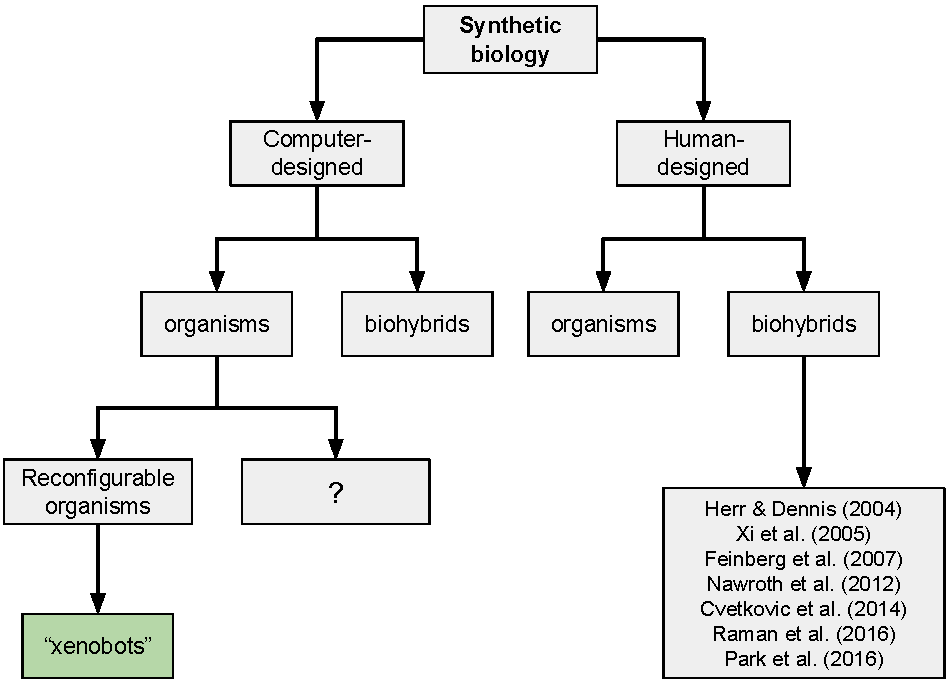
\includegraphics[width=\linewidth]{fig/synthbio.pdf}
    \vspace{1pt}
    \caption{%
    \textbf{Taxonomy of synthetic biology.}
    Xenobots are a specific kind of Reconfigurable Organism, which are a particular kind of Computer-Designed Organism, which is a particular mode of Synthetic Biology distinguished from human-designed biological constructs, which includes all organiods and biohybrids built to date.
    \label{fig:synthbio}%
    }
\end{figure}


\subsection{Future Work}

Despite our initial demonstrations that such is possible, 
it is still unclear which computer-designed organisms are easy, difficult or impossible to bioengineer in reality.
Computer-designed organisms are, in many ways, the inverse of traditional robots.
Many behaviors that are difficult to instantiate in robots composed of metal and electronics such as self assembly, -reconfiguration, -reproduction, and -repair, are ubiquitous in living materials.
On the other hand, we can fabricate just about any reasonably scaled and shaped structure using steel, concrete, or plastics; living systems tend to resist adopting new forms imposed on them.
The xenobots, as just one example, tend to smooth sharp edges and close small concavities in their sculpted body plans during development.

To more adequately investigate and exploit this strange inversion of engineering difficulty, contributions will need to span diverse academic departments: developmental biology, materials science, mechanical engineering, and computer science.



\section{Conclusion}

This thesis presented six sets of experiments (chapters 2, 3, 4, 5, 6 and 7), in which the morphologies of robots were permitted to vary on increasingly more scales in space and time.

